\documentclass[bigger]{beamer}
\usepackage[french]{babel}
\usepackage[utf8]{inputenc}
\usepackage[T1]{fontenc}
\usepackage{amsmath}
\usepackage{amsfonts}
\usepackage{amssymb}
\usepackage{graphicx}

\usebackgroundtemplate%
{%
    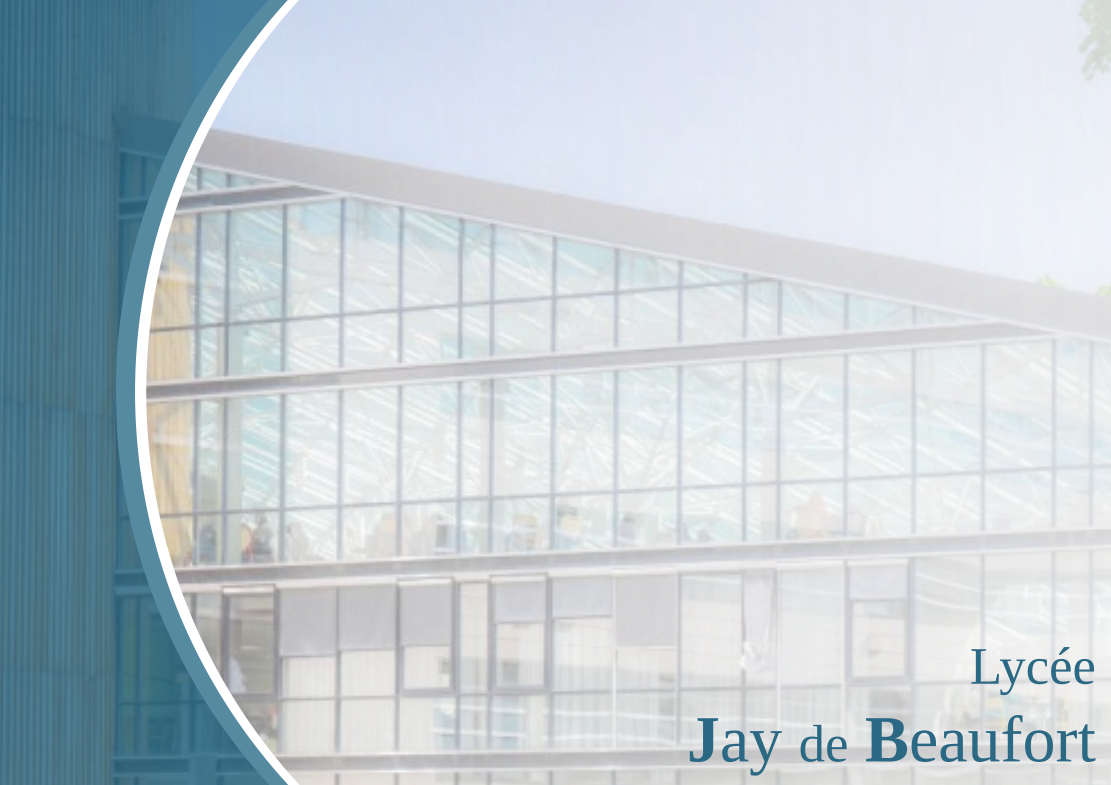
\includegraphics[width=\paperwidth,height=\paperheight]{ressources/plaquette-vierge.png}%
}

\title{Organisation Portes ouvertes}
\institute{Lycée Jay de Beaufort}
\date{jeudi 11 mars 2021}

\begin{document}
\frame{\titlepage}
\begin{frame}
\begin{center}
\Large{Inscription sur \url{https://lyceejaydebeaufort.fr}}
\centering
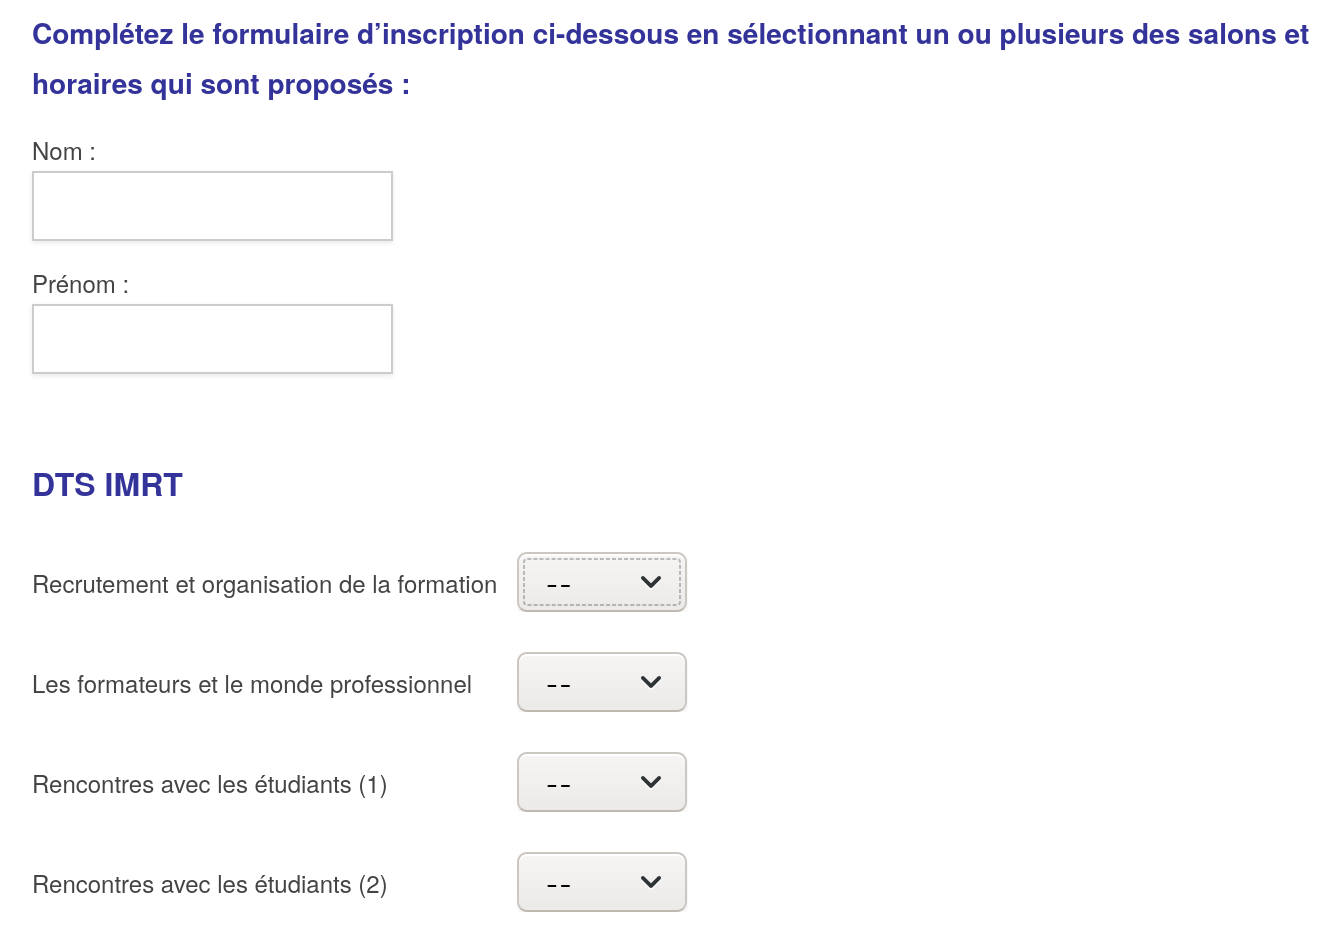
\includegraphics[width=7.5cm]{ressources/inscription.png}
\label{IMG}
\end{center}
\end{frame}

\begin{frame}
\begin{center}
    \begin{minipage}{0.6\textwidth}
    \Large Organisation \normalsize
      \begin{itemize}
      \item Définir les salons
      \item Définir les horaires
      \item Définir le nombre de participants
      \end{itemize}
    \end{minipage}
  \end{center}
\end{frame}
\begin{frame}
\begin{center}
\begin{minipage}{0.7\textwidth}
\Large Un salon \normalsize
      \begin{itemize}
      \item 20 minutes maximum
      \item 5-7 minutes de présentation
      \item 15 minutes de réponses aux questions
      \item Enseignant face caméra
      \item Un diaporama (2-3 slides)
      \item Une charte graphique commune
      \end{itemize}
    \end{minipage}
\end{center}
\end{frame}
\begin{frame}
\begin{center}
\begin{minipage}{0.5\textwidth}
\Large Outil \normalsize
      \begin{itemize}
      \item \url{https://meet.jit.si/}
      \item Chat
      \item Partage d'écran
      \end{itemize}
    \end{minipage}
\end{center}
\end{frame}

\end{document}